\documentclass{ctexbeamer}

\hypersetup{
  pdfcreator=TeX,
  pdfpagemode=FullScreen,
}

\mode<presentation>{
  \usetheme{Madrid}
  \setbeamertemplate{navigation symbols}{}
  \setbeamertemplate{footline}[frame number]
}

% -------------- 文档信息 --------------
\title{数据库大作业展示}
\subtitle{百货商店-图书管理系统}
\author{计试2201 梁佳伟 \and 计试2201 郑诗棪}
\institute[西安交大]{西安交通大学}
\date{2025年5月}
\subject{数据库课程展示}

\begin{document}

% 首页
\begin{frame}
  \titlepage
\end{frame}

% 目录
\begin{frame}{目录}
  \tableofcontents
\end{frame}

% 设计思想
\section{设计思想}

\subsection{整体设计思想}
\begin{frame}{整体设计思想}
  \begin{itemize}
    \item 构建百货商店管理后台,涵盖商品、库存、订单等功能
    \item 在此框架下,深入开发“图书管理系统”模块,面向用户呈现
    \item 图书系统支持:\pause
      \begin{itemize}
        \item 图书信息展示与分页浏览
        \item 多条件搜索(书名+作者)
        \item 可视化统计分类数据
        \item 购买需求清单(添加/删除)
      \end{itemize}
  \end{itemize}
\end{frame}

\subsection{百货商店概览}
\begin{frame}{百货商店概览}
  \begin{columns}
    \column{0.6\textwidth}
      \begin{itemize}
        \item 商品管理:增删改查、分类管理
        \item 库存监控:库存预警、批量入库
        \item 订单流程:下单、发货、退货
        \item 用户与权限:登录、角色分配、日志记录
      \end{itemize}
    \column{0.8\textwidth}
      % \begin{figure}
      %   \centering
      %   % ER 图示例
      %   \includegraphics[width=0.9\textwidth]{fig/store_er.png}
      %   \caption{百货商店 ER 图}
      % \end{figure}
  \end{columns}
\end{frame}

\subsection{图书管理系统}
\begin{frame}{图书管理系统}
  \begin{itemize}
    \item 爬虫从豆瓣获取约3万条图书数据
    \item 存储字段:书名、作者、分类、价格、页数、评分、简介、详情链接
    \item 用户可:搜索、浏览、查看详情、添加“购买需求”、查看&删除需求
    \item 支持分类统计与可视化展示
  \end{itemize}
  \vspace{0.3cm}
  \begin{figure}
    \centering
    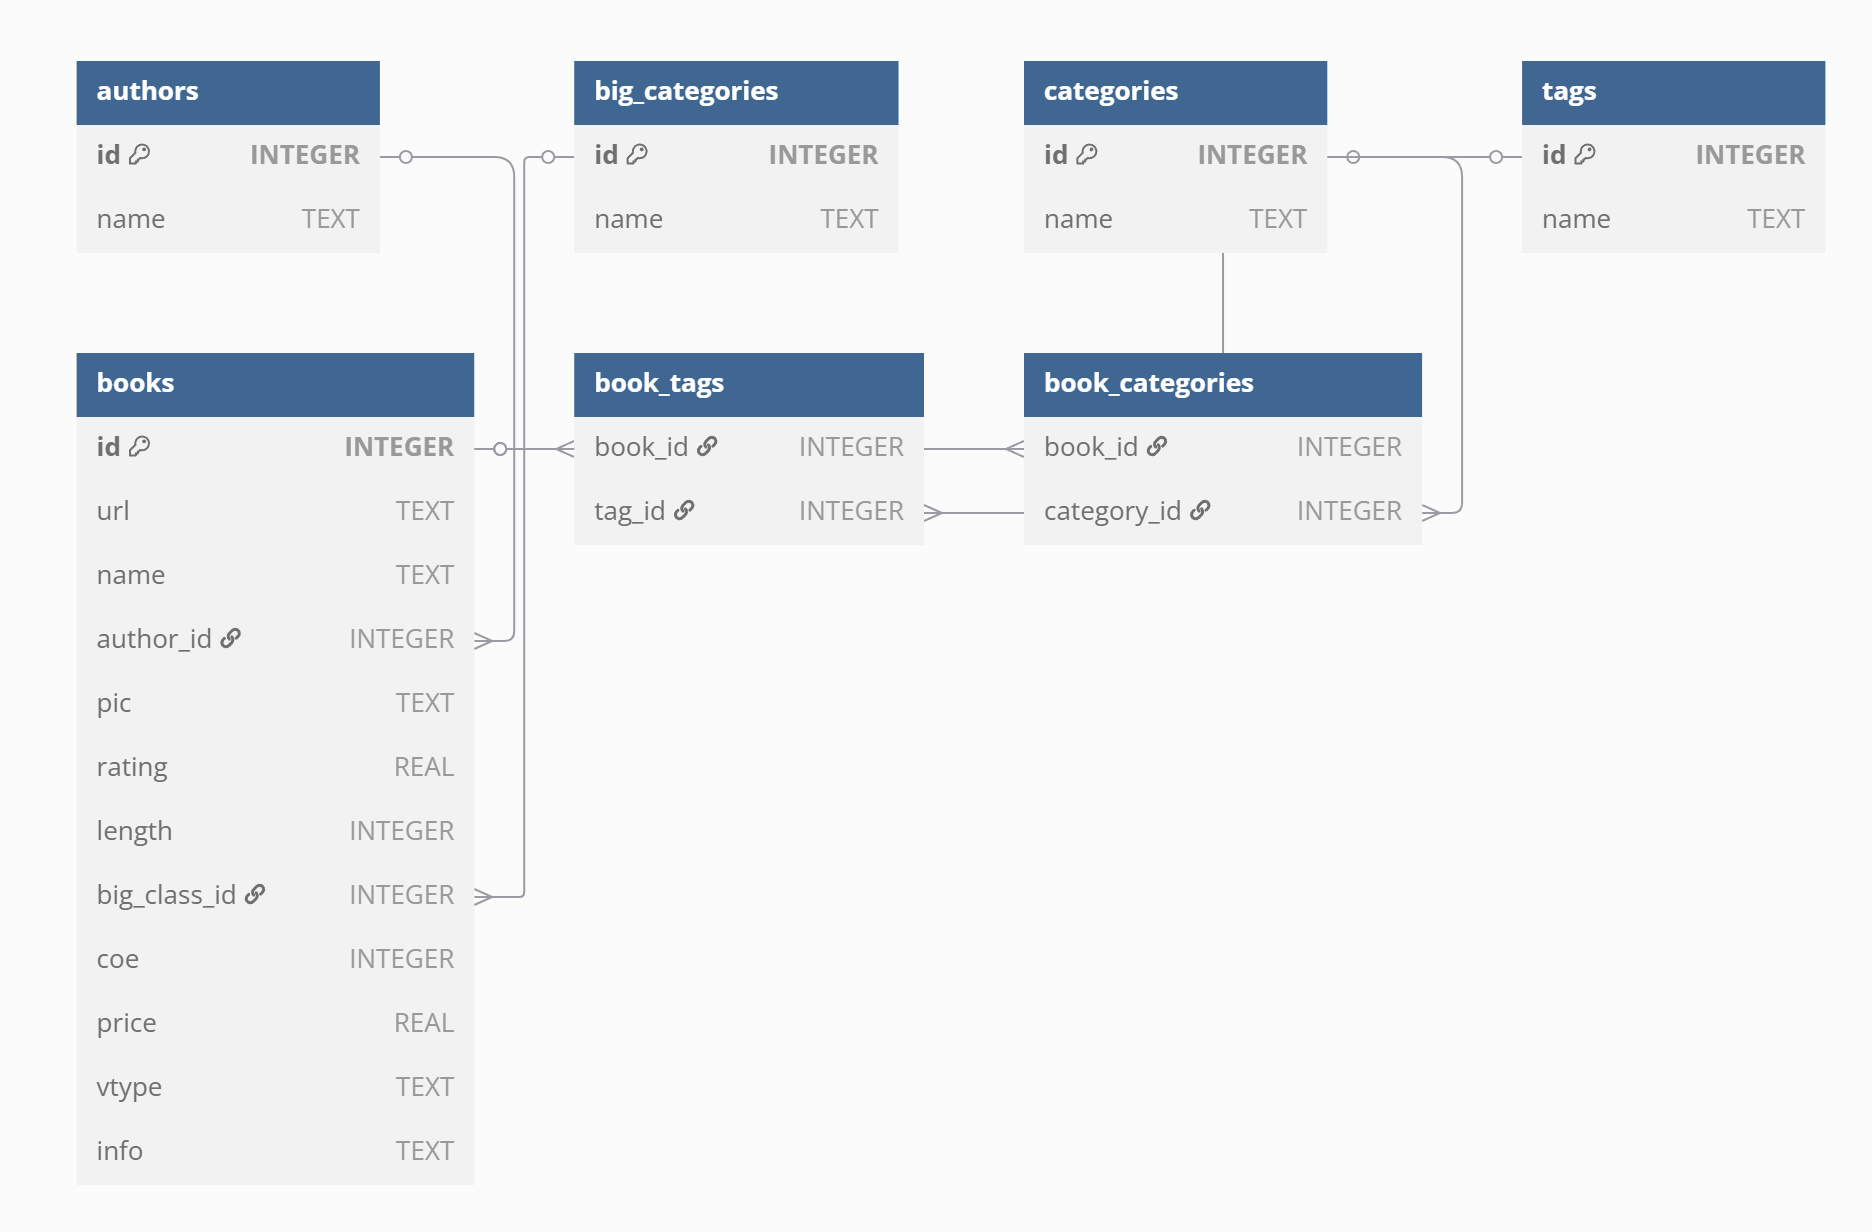
\includegraphics[height=3cm]{fig/bookER.png}
    \caption{图书 JSON 示例 \quad 图书 ER 图}
  \end{figure}
\end{frame}

% 前端展示
\section{前端展示}

\subsection{百货商店入口}
\begin{frame}{百货商店入口}
  % \begin{figure}
  %   \centering
  %   \includegraphics[width=0.7\textwidth]{fig/store_home.png}
  %   \caption{百货商店后台首页}
  % \end{figure}
\end{frame}

\subsection{百货商店部分功能}
\begin{frame}{百货商店部分功能}
  % \centering
  % 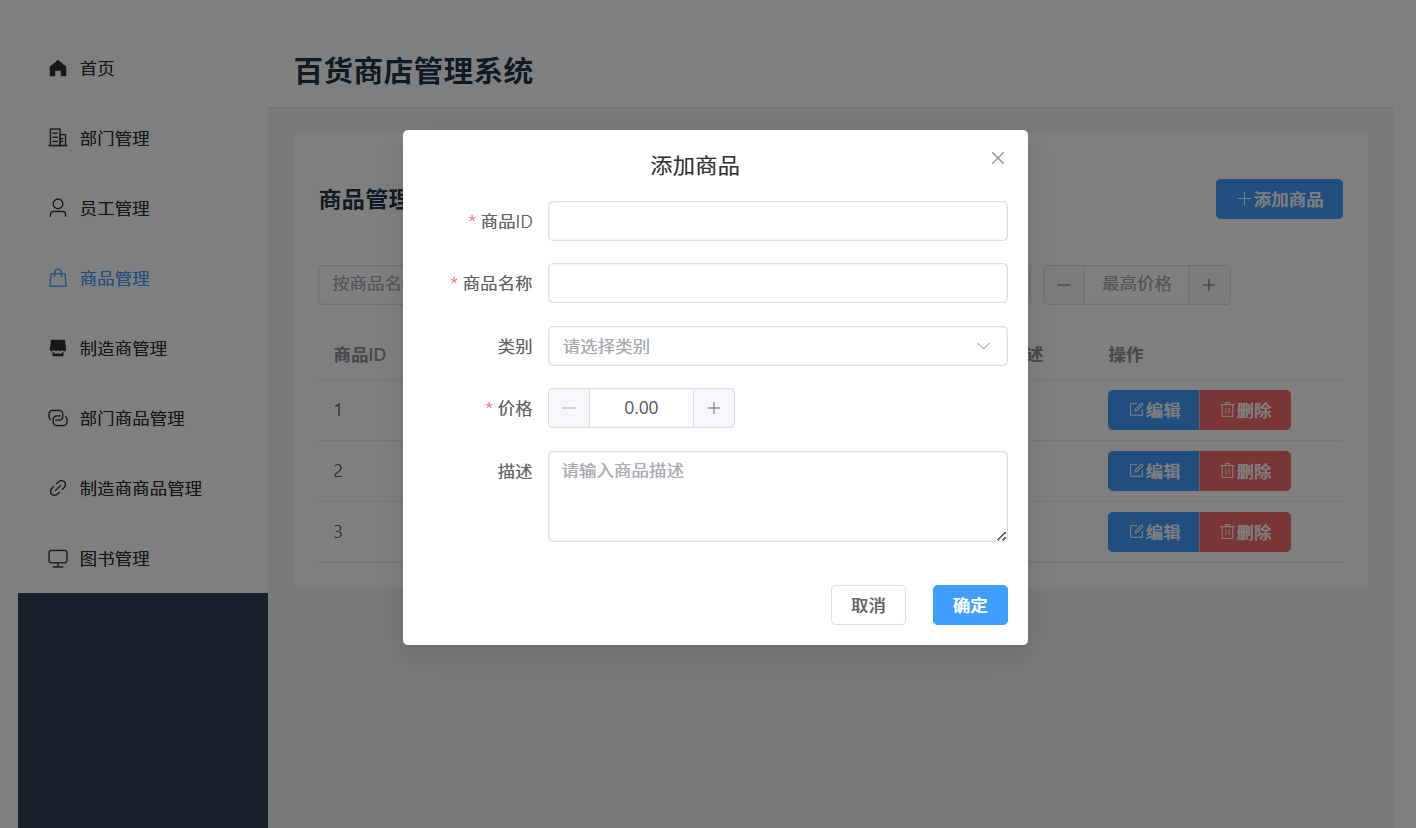
\includegraphics[width=0.45\textwidth]{fig/store_goods.png}
  % \hspace{0.5cm}
  % \includegraphics[width=0.45\textwidth]{fig/store_order.png}
  % \vspace{0.3cm}
  % \\textit{商品管理界面} \quad \textit{订单列表界面}
\end{frame}

% 图书管理系统前端
\subsection{图书管理系统部分功能}
\begin{frame}{图书管理系统部分功能}
  \centering
  \begin{minipage}{0.45\textwidth}
    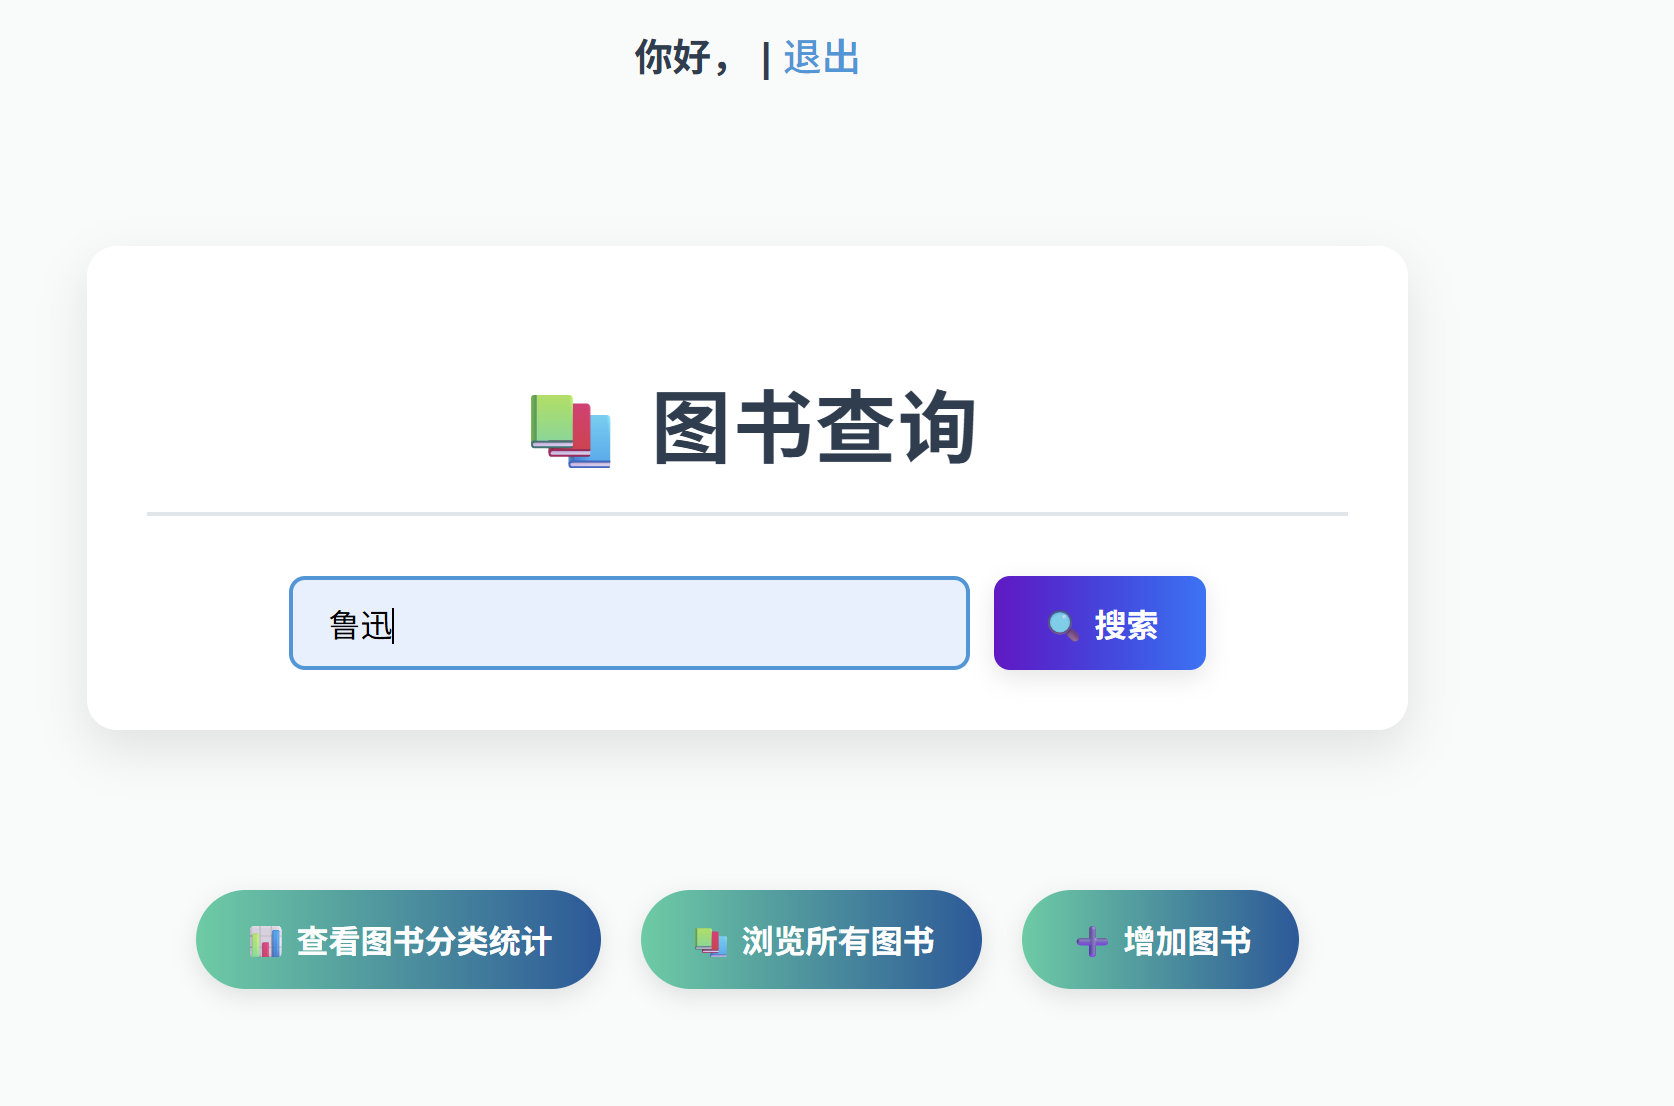
\includegraphics[width=\textwidth]{fig/book1.png}\\ 图书列表与分页
  \end{minipage}
  \begin{minipage}{0.45\textwidth}
    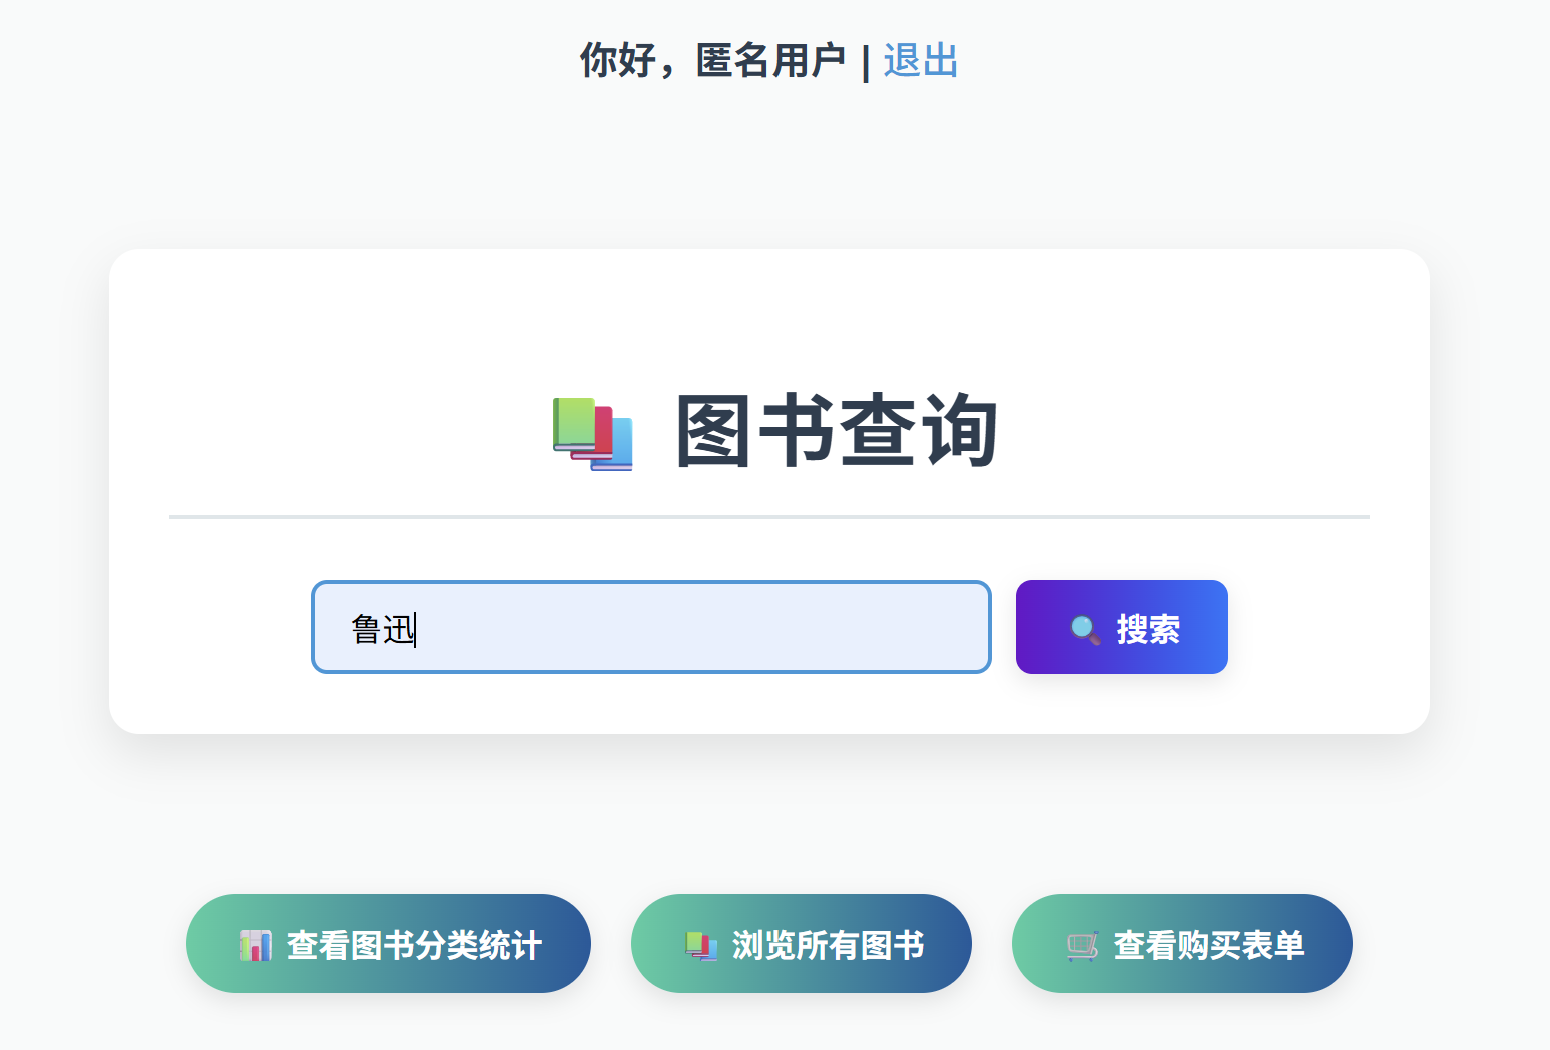
\includegraphics[width=\textwidth]{fig/book2.png}\\ 搜索图书
  \end{minipage}
  \vspace{0.3cm}
  \begin{minipage}{0.45\textwidth}
    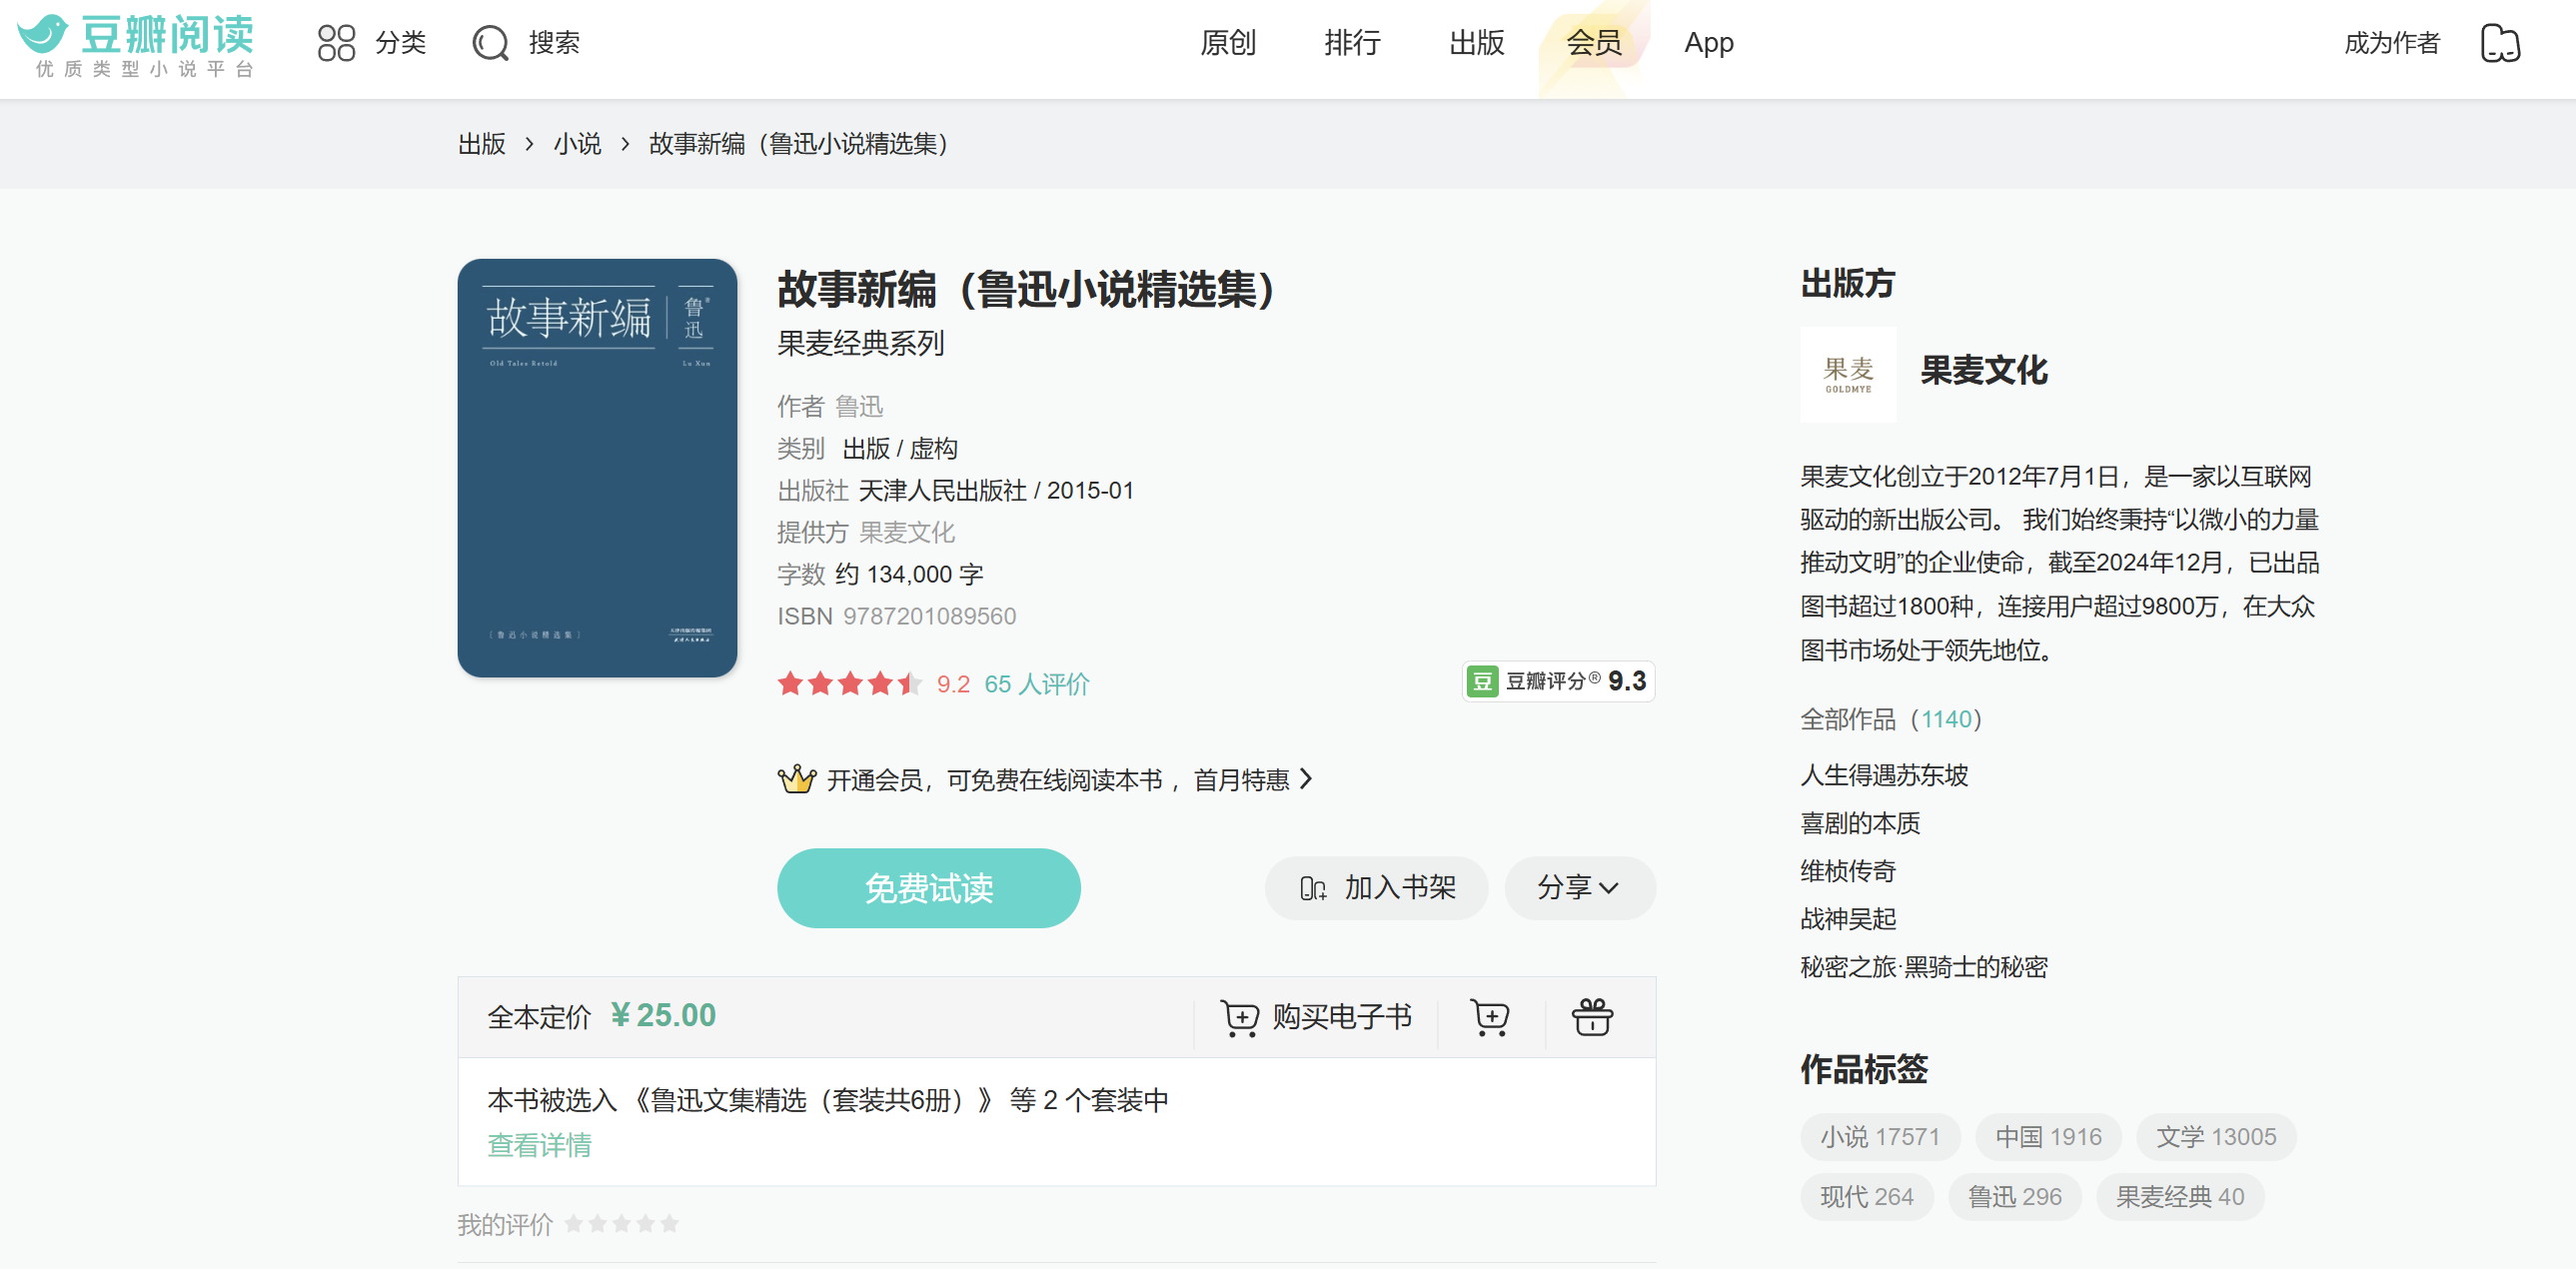
\includegraphics[width=\textwidth]{fig/book3.png}\\ 详情跳转
  \end{minipage}
  \begin{minipage}{0.45\textwidth}
    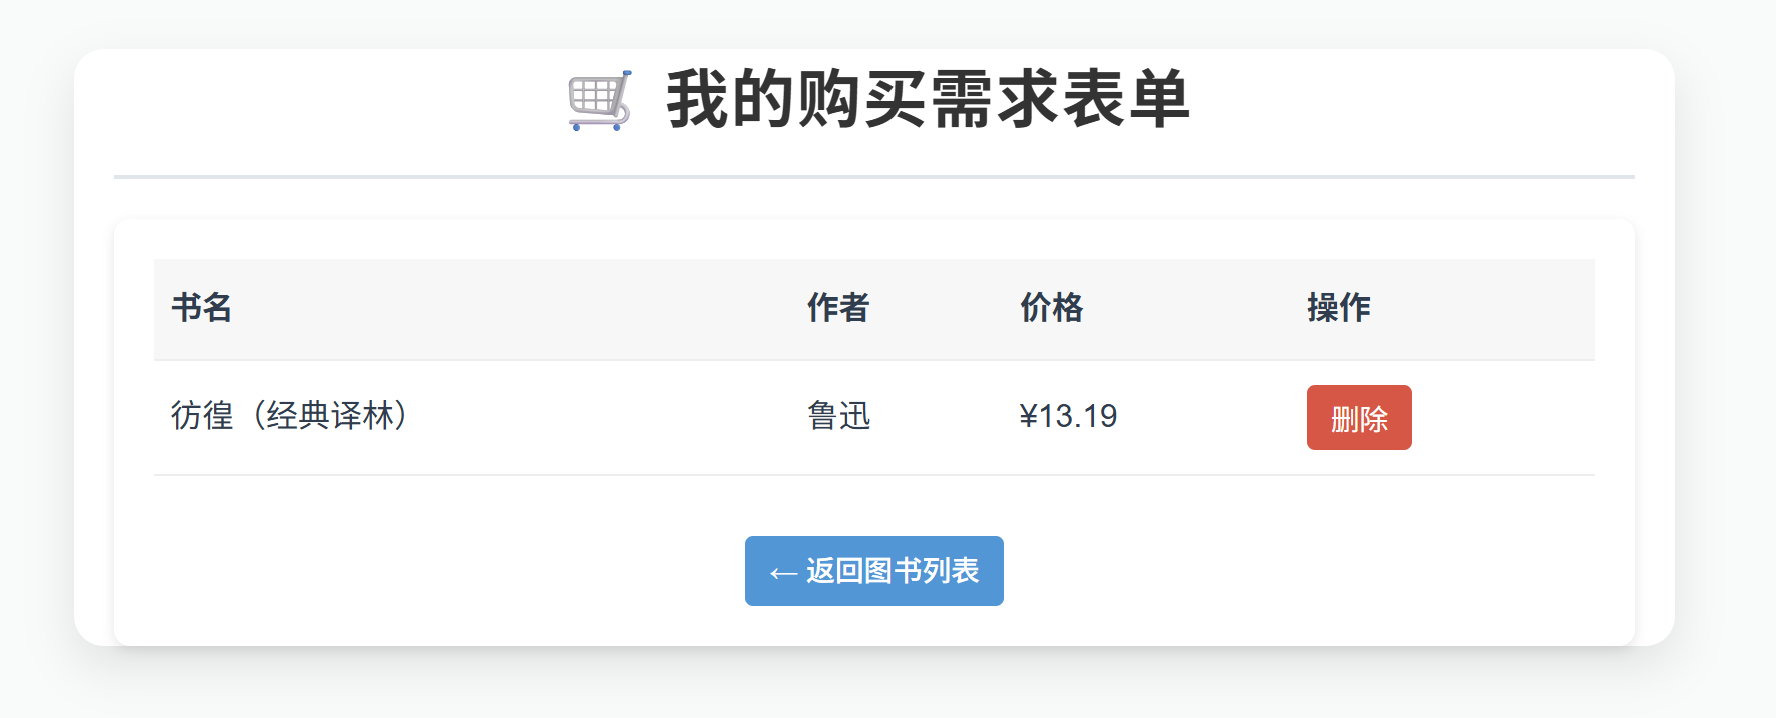
\includegraphics[width=\textwidth]{fig/book4.png}\\ 添加购买需求
  \end{minipage}
\end{frame}

\begin{frame}{图书管理系统更多功能}
  \centering
  \begin{minipage}{0.45\textwidth}
    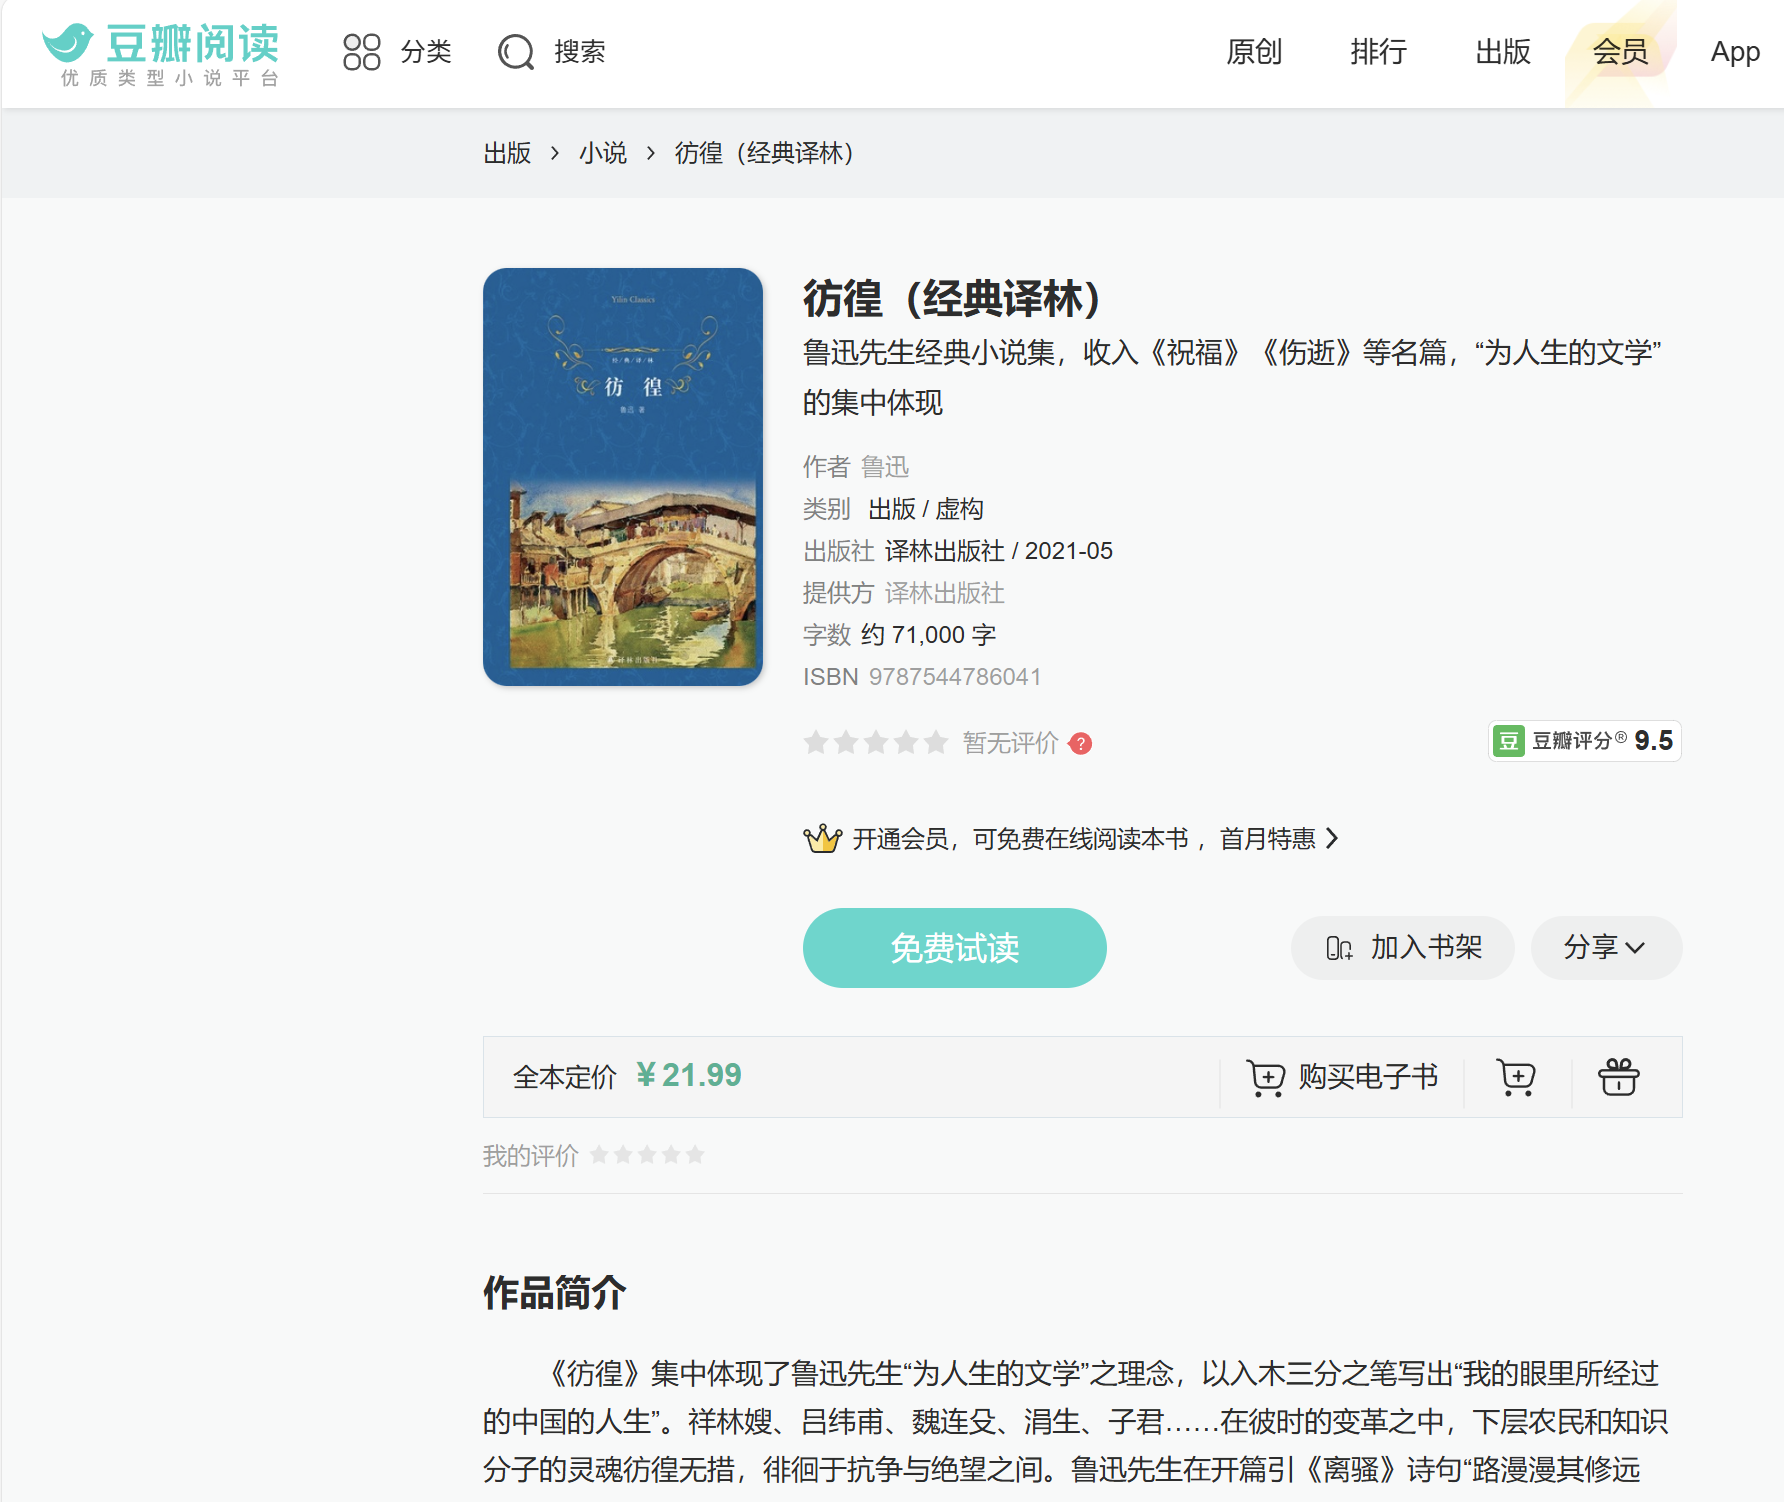
\includegraphics[width=\textwidth]{fig/book5.png}\\ 购买清单查看
  \end{minipage}
  \begin{minipage}{0.45\textwidth}
    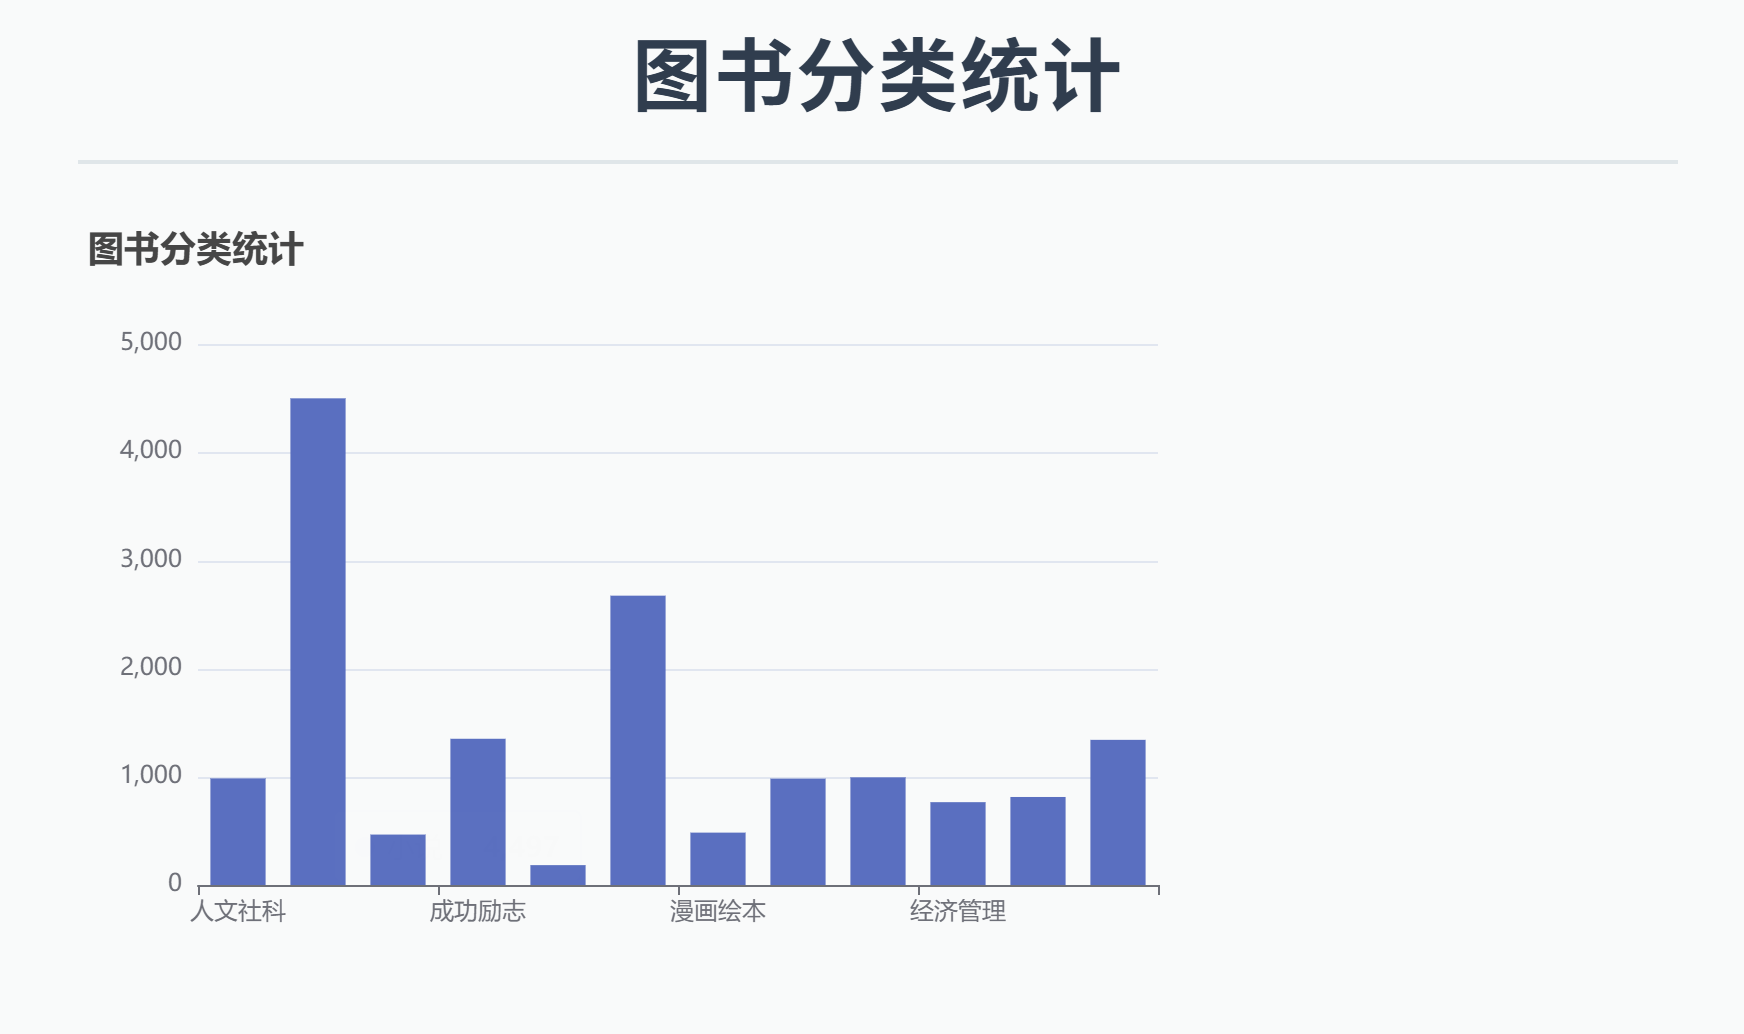
\includegraphics[width=\textwidth]{fig/book6.png}\\ 分类统计可视化
  \end{minipage}
  \vspace{0.3cm}
  \begin{itemize}
    \item 用户点击图书可跳转至豆瓣页面获取详细信息
    \item 使用 ECharts 生成图书分类柱状图,直观呈现图书分布
  \end{itemize}
\end{frame}

% 后端思路
\section{后端思路}

\subsection{数据库设计}
\begin{frame}{数据库设计}
  \begin{itemize}
    \item 核心表:\texttt{books}, \texttt{authors}, \texttt{big_categories}, \texttt{purchase_requests}
    \item 主外键关系:\\
      \texttt{books.author\_id} \ensuremath{\to} \texttt{authors.id}\\
      \texttt{books.big\_class\_id} \ensuremath{\to} \texttt{big_categories.id}\\
      \texttt{purchase\_requests.book\_id} \ensuremath{\to} \texttt{books.id}
    \item 购书需求记录附带 \texttt{username} 与时间戳
  \end{itemize}
\end{frame}

\subsection{Python–Flask 实现}
\begin{frame}{Python–Flask 实现}
  \begin{itemize}
    \item 使用 \texttt{Flask} 与 \texttt{sqlite3} 实现后端服务
    \item 统一数据库连接 & 事务管理:\texttt{get\_db()}, \texttt{teardown\_appcontext}
    \item 路由设计:
      \begin{itemize}
        \item \texttt{/books}:分页浏览
        \item \texttt{/search}:模糊搜索
        \item \texttt{/add\_to\_purchase/<book\_id>}:添加购买需求
        \item \texttt{/purchase\_list}:查看 \& 删除需求
      \end{itemize}
    \item 登录无需密码,仅录入用户名并创建需求表
  \end{itemize}
\end{frame}

\end{document}

